\documentclass[a4paper,twoside,12pt,DIV=13,BCOR=5mm,numbers=noenddot,cleardoublepage=empty]{scrbook}
\input{format-LU} 
\usepackage{ucs} 	
\usepackage{float}		% File mit den ben�tigten Packeten, den Formatanweisungen und den Befehlsdefinitionen
\usepackage{graphicx}
\begin{document}
\newcommand\todo[1]{\textcolor{red}{#1}}
%=============================================================================================
% Titelblatt und Inhaltsverzeichnis
%=============================================================================================
\renewcommand{\baselinestretch}{1.25}
\newcommand{\StudentA}{Marton Harsch}
\newcommand{\MatrNrA}{12123680}
\newcommand{\StudentB}{Michael Malburg}
\newcommand{\MatrNrB}{61806515}
\newcommand{\StudentC}{Jonathan Gamperl}
\newcommand{\MatrNrC}{12302766}

\newcommand{\LUDatum}{22.4.2024}
\newcommand{\LUGruppe}{}
\newcommand{\LUBetreuer}{}

\large
\includepdf[fitpaper=true,
						picturecommand*={\unitlength1cm 
						\put(7.3,7.7){\StudentA} \put(14.1,7.7){\MatrNrA}
            \put(7.3,7.0){\StudentB} \put(14.1,7.0){\MatrNrB}
            \put(7.3,6.3){\StudentC} \put(14.1,6.3){\MatrNrC}
						\put(7.3,5.1){\LUDatum} 
            \put(7.3,4.4){\LUGruppe} 
            \put(7.3,3.7){\LUBetreuer} 
}]
{pictures/DeckblattLUDie}     %file name of title page


%===============================================================================
% Text
%===============================================================================

\cleardoublepage
\setcounter{tocdepth}{3}

\setcounter{page}{0}
\renewcommand{\thepage}{\roman{page}}
\tableofcontents \cleardoublepage

\setcounter{page}{1}
\renewcommand{\thepage}{\arabic{page}}
\setcounter{chapter}{0}


%===============================================================================

\newpage
\chapter{Zusammenfassung}
Die Zusammenfassung
\newpage
\chapter{Ringkerntrafo}
\section{Aufnahme einer Hystereseschleife}

\section{Aufnahme der Permeabilit\"atskurve}
\subsection{Hintergrund}
Wird aus der Schaltung zur Aufnahme der Hystereseschleife der Integrator entfernt, steht die gemessene Spannung nicht mehr in Proportion 
zum Fluss durch die Spule, sondern zu seiner \"anderungsrate. In diesem Fall kann das Entfernen des Integrators mit dem Ableiten der Funktion
gleichgesetzt werden. Betrachten wir das Verh\"altnis aus der Feldst\"arke und der \"anderungsrate der Flussdichte sprechen wir von 
differenzieller Permeabilit\"at. Wird diese noch durch die Permeabilit\"at des Vakuums geteilterhalten wir die relative differenzielle Permeabilit\"at Ziel ist es diese zu messen 
und mit der Hystereseschleife auf plausibilit\"at zu pr\"ufen, sowie ihren spitzenwert zu finden.
\subsection{Messergebnisse}
\begin{figure}
  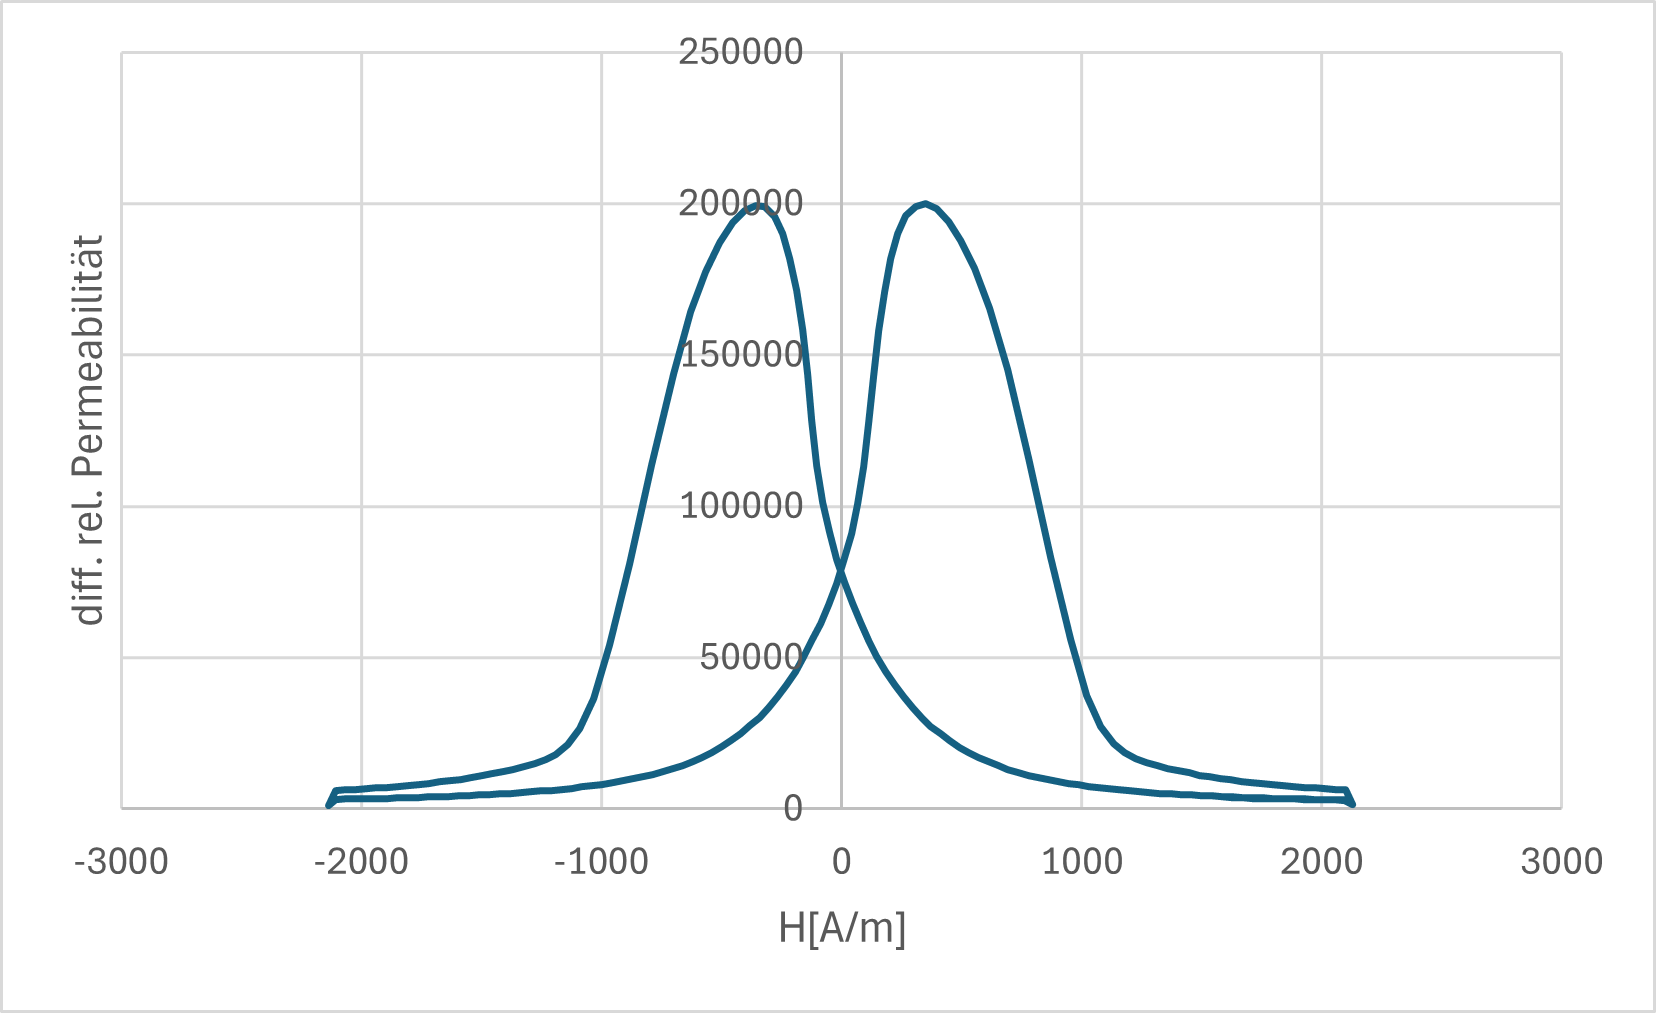
\includegraphics[width=\linewidth]{pictures/Permeabilitaet.png}
  \caption{Differenzielle relative Permeabilit\"at abh\"angig von der Feldst\"arke.}
  \label{fig:perm}
\end{figure}
Das Diagramm \ref{fig:perm} zeigt die gemessene differenzielle relative Permeabilit\"at abh\"angig von der Feldst\"arke. Verglichen mit der Hystereseschleife ist die steigungs\"anderung an sich plausibel, der H\"ochstwert an sich mit fast 200.000 doch etwas fragw\"urdig.

\section{Hysteresefamilie und Entmagnetisierung}
\label{Entmag}
\subsection{Setup}
Um die Neukurve (siehe \ref{Neukurve}) aufnehmen zu k\"ofnnen, braucht es einen unmagnetisierten Werkstoff. 
Der Ringkern wird dazu wiederholt, immer schw\"acher werdend ummagnetisiert wobei die Remanenz jedes mal kleiner wird.
Die dabei entstehende zusammensetzung aus schw\"acher werdenden Hystereseschleifen wird als Hystesresefamilie bezeichnet. 
Um einen kontinuierlich schw\"acher werdenden Sinusstrom durch die Elektromagneten zu schicken wird das Signal des Funktionsgenerators 
mit der Spannung eines sich entladenden Kondendsators moduliert. Der Funktionsgenerator liefert unmoduliert eine Sinusspannung von 6Vpp mit einer Periodendauer von 10s.
Die RC Schaltung mit deren Spannung die des Funktionsgenerators moduliert wird besitzt eine Zeitkonstante von 60s. Die  induzierte Spannung an der Messpule wird f\"ur diese Messung integriert. 
Die Widerstandswerte bleiben gleich.
\subsection{Messergebnisse}
\begin{figure}
  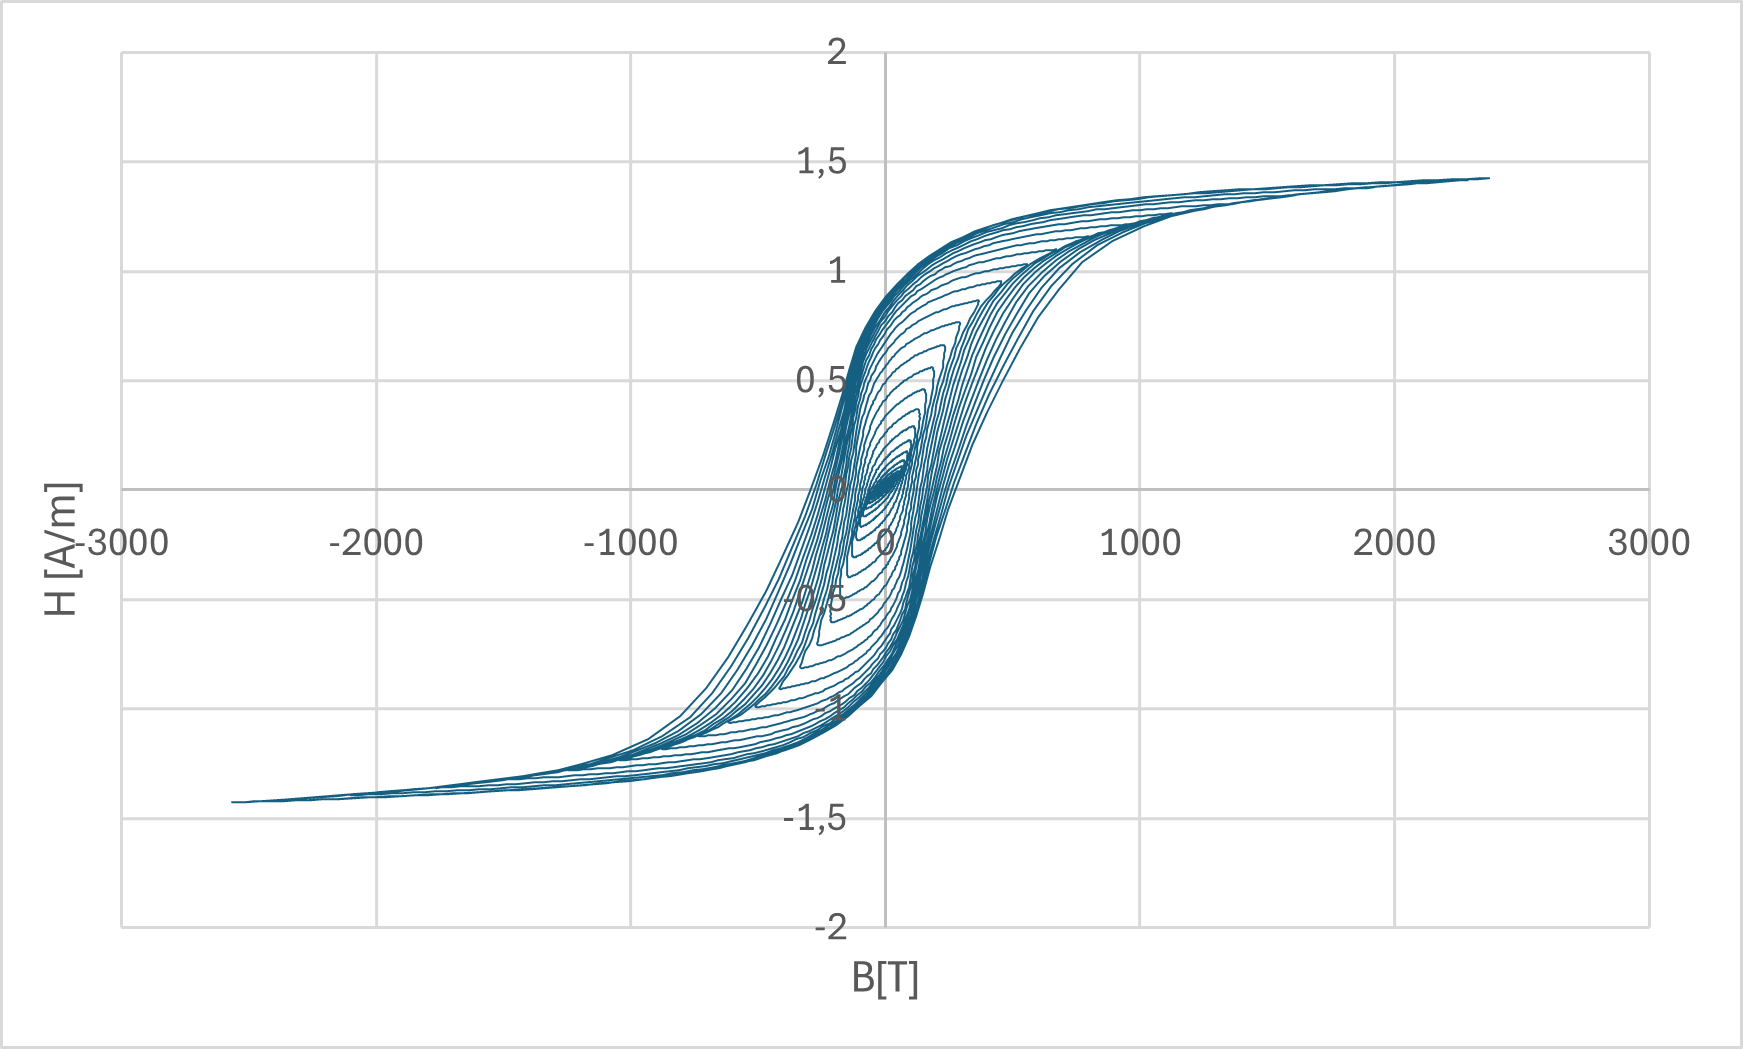
\includegraphics[width=\linewidth]{pictures/Hysteresefamilie.png}
  \caption{Hysteresefamilie die die Entmagnetisierung des Ringkerns zeigt.}
  \label{fig:entmag}
\end{figure}
In dem Diagramm \ref{fig:entmag} kann sch\"ofn die Entmagnetisierung des Materials durch die immer kleiner werdenden Hystereseschleifen betrachtet werden.

\section{Die Neukurve}\label{Neukurve}
\subsection{Setup}
Ziel dieser Messung ist es eine Hystereseschleife inklusive einer Neukurve aufzunehmen. 
Dazu wird der gleiche Messaufbau wie beim einfachen Messen der Hystereseschleife verwendet. Anders ist in diesem Fall aber, dass der Kern des Trafos entmagnetisiert wurde (siehe \ref{Entmag}) und 
die Dreiecksspannung nur als zwei Zyklen Burst angelegt wird.
\subsection{Messergebnisse}
\begin{figure}
  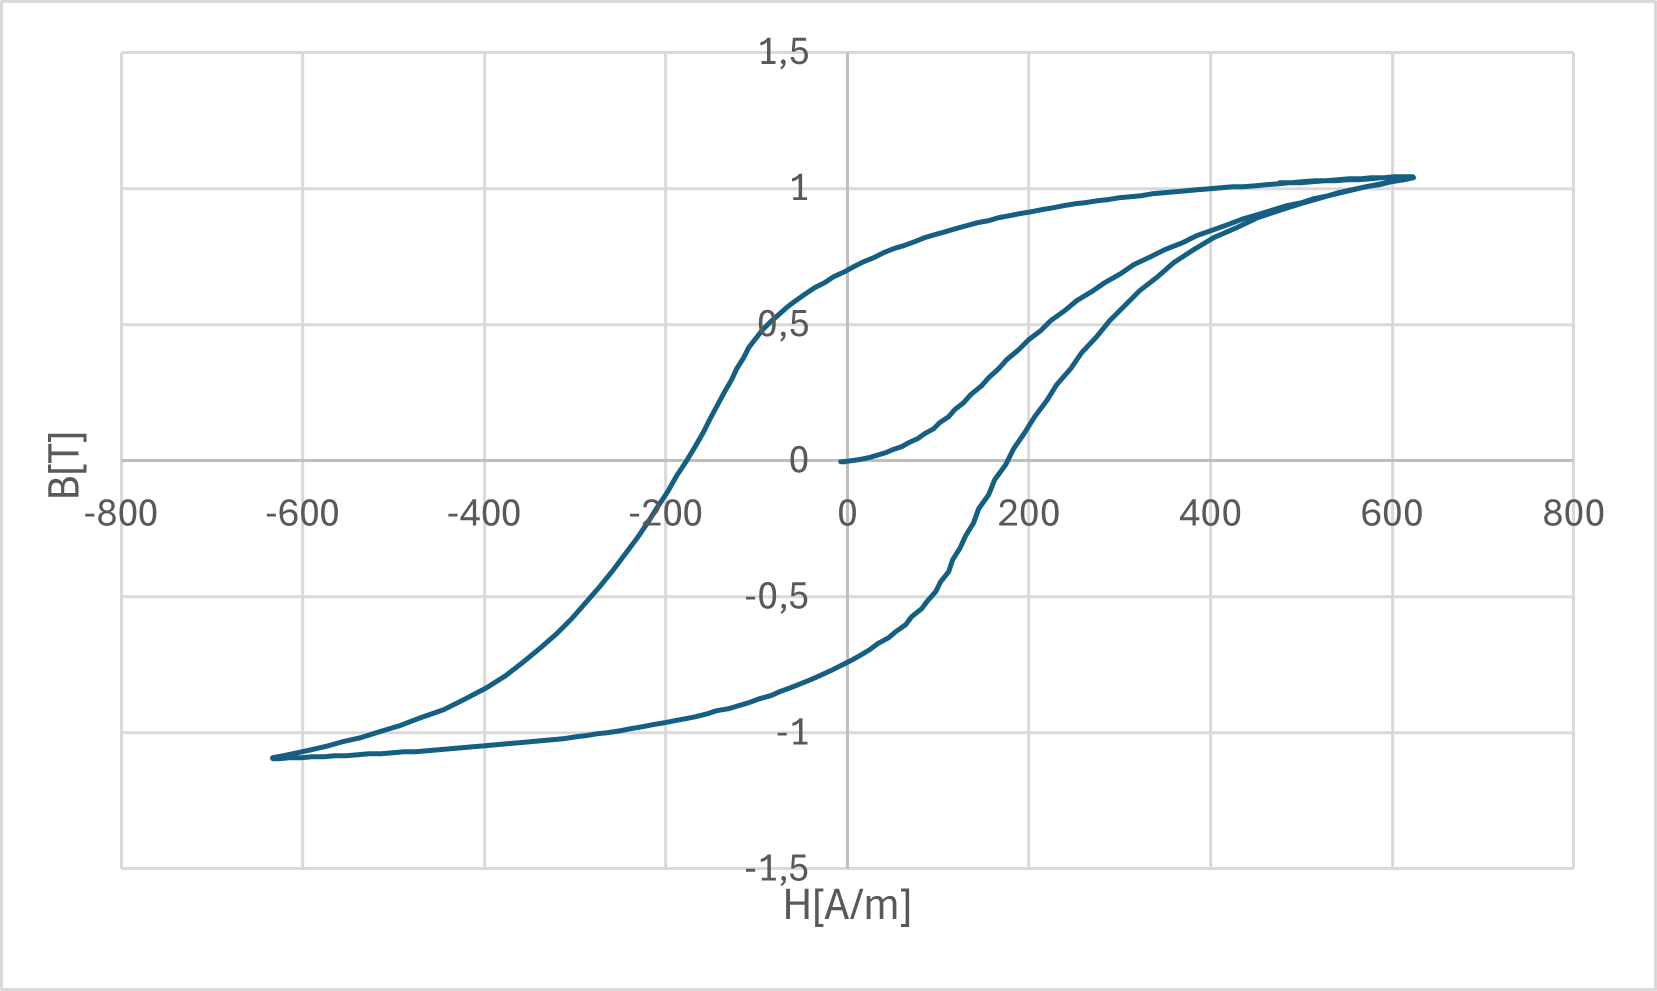
\includegraphics[width=\linewidth]{pictures/Neukurve.png}
  \caption{Hystereseschleife mit Neukurve.}
  \label{fig:neukurve}
\end{figure}
Im Diagramm \ref{fig:neukurve} sehen wir die bereits bekannte Hystereseschleife mit einer zus\"atzlichen Neukurve die das initale Magnetisieren des unmagnetisierten Stoffes darstellt.
\chapter{\"ubungen am Elektromagneten}
\section{Metallscheiben im Magnetfeld}

\section{Eisenblech im Magnetfeld}

\section{Diamagnetische Stoffe}

\section{Messung des Magnetfeldes}

\section{Lorentzkraft}

´\section{Fazit}



\subsection{Messung} 



\end{document}


